\documentclass{article}

\usepackage[utf8]{inputenc}
\usepackage{amssymb}
\usepackage{amsmath} 
\usepackage{enumitem}
\usepackage{pgf,tikz}
\usepackage{tkz-euclide}
\usepackage{mathrsfs}
\usepackage{xcolor}
\usetikzlibrary{arrows}
\usepackage{fancyhdr}
\usepackage{hyperref}
\usepackage{wrapfig}
\usepackage{polski}
\usepackage{gensymb}
\usepackage[many]{tcolorbox}

% definicja koloru
\definecolor{kolor}{RGB}{8, 97, 138}

\DeclareUnicodeCharacter{2212}{-}

% definicja kąta
\def\an{\hbox{\lower-.2ex\hbox{$<\kern-.53em)$}$\,$}}

\usepackage[b5paper, left=0.8in, right=0.8 in, top=0.8 in, bottom=0.8 in]{geometry}

\usetikzlibrary{arrows, calc,intersections, decorations.pathmorphing}
\tikzset{
arrowMe/.style={postaction=decorate,
    decoration={markings, mark=at position .5 with {\arrow[thick]{#1}}
    } }}


\newcommand{\heading}[1]{
	\noindent
	\textbf{\textcolor{kolor}{#1}}
	\vspace{5px}
}

\newcommand{\remark}{
	\noindent\textit{Uwaga}\\
}

\newcommand{\theory}[1]{
	\begin{center}
    \fontsize{26}{20}\selectfont
	\textbf{\textcolor{kolor}{#1}}
	\end{center}
	\vspace{20px}
}

\tcbset{mystyle/.style={
  breakable,
  enhanced,
  outer arc=0pt,
  arc=0pt,
  colframe=kolor,
    coltitle=kolor,
  colback=white,
  attach boxed title to top left={yshift=-2mm},
  boxed title style={
    coltitle=kolor,
    colback=white,
    outer arc=0pt,
    arc=0pt,
    top=3pt,
    bottom=3pt,
    },
  fonttitle=\sffamily
  }
}

\newtcolorbox[auto counter]{problem_box}[1][1]{
  mystyle,
  title=Zadanie~{#1},
}


\newlist{hints_list}{enumerate}{3}

\setlist[hints_list]{label=\textbf{\textcolor{kolor}{\arabic*}}.}

\newcommand{\hints}[1]{
	\begin{center}
    \fontsize{20}{20}\selectfont
	\textbf{\textcolor{kolor}{#1}}
	\end{center}
}

\newcommand{\solutions}[1]{
	\begin{center}
    \fontsize{26}{20}\selectfont
	\textbf{\textcolor{kolor}{#1}}
	\end{center}
	\vspace{20px}
}


\newenvironment{problem}[1]
{
    \begin{samepage}
    \begin{problem_box}[{#1}]
}
{ 
    \end{problem_box}
    \end{samepage}
}

\newcommand{\answer}[1]{
  \noindent\textit{Odpowiedź.} #1
  \vspace{5px}
}



\begin{document}

\thispagestyle{empty}\addtocounter{page}{-1}
%\vspace*{\fill}
	\begin{center}
		\fontsize{15}{15}\selectfont
		Paweł Gadziński

		\vspace{50px}

		\fontsize{40}{40}\selectfont
		\textcolor{kolor}{Wstęp do matematyki olimpijskiej}

		\vspace{20px}

		\fontsize{25}{25}\selectfont
		\textcolor{kolor}{zadania niegeometryczne}

		\vspace{40px}

		\fontsize{15}{15}\selectfont
		wersja z 29 lipca 2021
	\end{center}
\vspace*{\fill}
\begin{center}
		\fontsize{15}{15}\selectfont
		Książka w wersji online dostępna pod adresem: \\
		\url{http://wdmo.pl}
\end{center}
\newpage
	\vspace*{\fill}
	\begin{center}
		\addcontentsline{toc}{section}{Wstęp}
		\fontsize{20}{20}\selectfont
		\textbf{Wstęp}
		\vspace{30px}
	\end{center}
		\noindent
		Książka ta jest skierowana do osób, które mają już pewne doświadczenie z matematyką olimpijską i chcieliby powalczyć o tytuł finalisty Olimpiady Matematycznej. Jeśli czytelniczka/czytelnik nie ma takowego doświadczenia, to zachęcamy, aby najpierw zapoznać się z zadaniami i materiałami z Olimpiady Matematycznej Juniorów.

		\vspace{10px}
		\noindent
		Każdy z rodziałów zaczyna się omówieniem pewnego zagadnienia teoretycznego. Postaram się zamieścić w tej książce wszystkie niezbędne narzędzia, które moga przydać się na drugim etapie OM. 

		\vspace{10px}
		\noindent
		Jednak to nie wiedza teoretyczna jest najważniejsza na Olimpiadzie. Znacznie istotniejsze jest jej kreatywne zastosowanie, często wykraczające poza schematy. Dlatego częścią każdego rozdziału jest kilka zadań. Są one dobrane tak, aby były niesztampowe oraz poszerzały horyzonty myślowe. Absolutnie nie należy traktować ich jako ćwiczeń do poprzedzającej ich części teoretycznej. Mogą one do niej nawiązywać, ale nie zawsze będą. Trenowanie na zadaniach, które są bardziej zróżnicowane pod względem tematyki jest bardziej efektywne, czego dowodzą liczne badania prowadzone w tym zakresie(Roher, Dedrick i Burgess, 2014). 

		\vspace{10px}
		\noindent
		Do każdego z zadań zamieszczono do trzech podpowiedzi. Zachęcamy do skorzystania z nich przed zobaczeniem na rozwiązanie. Przy większości zadań przeczytanie wszytskich podpowiedzi powinno pozwolić na samodzielne wymyślenie rozwiązania, a to daje satysfakcję.

		\vspace{10px}
		\noindent
		Książka jest dostępna za darmo, ale jednak proszę osoby, które z niej korzystają o drobną przysługę. Jeśli zostanie zauważony jakiś błąd, nieścisłość, czy też uważasz, że można coś napisać lepiej, to bardzo prosiłbym o zwrócenie uwagi przez formularz dostępny w wersji on-line publikacji lub też pisanie na maila \textit{admin@wdmo.pl}.

		\vspace{10px}
 
		\hspace*{\fill}Paweł Gadziński

\vspace*{\fill}
\newpage

\newpage
\headingpage{Teoria i zadania}

% Rozdział 1 – indukcja matematyczna

\theory{Indukcja matematyczna}

\heading{Przykład 1}

\noindent
Wykazać, że dla każdej liczby dodatniej całkowitej $n$ zachodzi nierówność
\[
	2^n \geqslant n + 1.
\]

\heading{Rozwiązanie}

\noindent
Dla $n = 1$ mamy $2^n = 2 = n + 1,$ a więc postulowana nierówność istotnie zachodzi.
Załóżmy, że dla pewnej liczby dodatniej całkowitej $k$ zachodzi nierówność ${2^k \geqslant k + 1}$. Zauważmy, że wówczas
\[
	2^{k + 1} = 2 \cdot 2^k \geqslant 2 \cdot (k + 1) = 2k + 2 \geqslant k + 2.
\]

\noindent
Wykazaliśmy, że jeśli postulowana nierówność zachodzi dla pewnej dodatniej liczby całkowitej $k$, to zachodzi również dla liczby $k + 1$. Skoro zachodzi ona dla $n = 1$, to zachodzi również dla $1 + 1 = 2,\; 2 + 1 = 3,\; 3 + 1 = 4, ...$ -- wszystkich liczb naturalnych.

\qed

\vspace{10px}

\noindent
Alternatywnym, ale równoważnym, sposobem zakończenia rozwiązania powyższego przykładu jest rozpatrzenie najmniejszego naturalnego $n$, dla którego teza nie zachodzi. A więc dla $n - 1$ nierówność musi zachodzić, chyba że $n = 1$. Ale w tym przypadku sprawdzamy, że teza zachodzi. Skoro dla $n - 1$ teza jest prawdziwa, a dla $n$ już nie, to otrzymujemy sprzeczność z wcześniej poczynioną obserwacją.

\vspace{10px}
\heading{Zasada indukcji matematycznej}

\noindent
Metodę dowodzenia zastosowaną w ostatnim akapicie powyższego rozwiązania nazywamy \textit{zasadą indukcji matematycznej}.
Formalizując, dowód indukcyjny zdania logicznego $Z(n)$ dla dowolnej dodatniej liczby całkowitej $n$ składa się z dwóch części:
\begin{enumerate}
	\item Baza indukcji -- sprawdzenie prawdziwości zdania $Z(1)$.
	\item Krok indukcyjny -- udowodnienie, że jeśli zachodzi zdanie $Z(k)$, to zachodzi $Z(k + 1)$.
\end{enumerate}


\noindent
Indukcję matematyczną da się wykorzystać poza algebrą. Pokażemy jedno jego zastosowanie kombinatoryczne. Ale najpierw musimy zdefiniować kilka pojęć z teorii grafów.

\vspace{20px}

\heading{Grafy i ścieżki Hamiltona}

\vspace{5px}

\noindent
\textit{Grafem} nazywamy pewien zbiór \textit{wierzchołków} na płaszczyźnie, które są połączone \textit{krawędziami}. \textit{Ścieżką} nazywamy ciąg parami różnych krawędzi pewnego grafu, z których dwie kolejne mają wspólny wierzchołek. \textit{Ścieżką Hamiltona} nazywamy ścieżkę, która przechodzi przez każdy wierzchołek dokładnie raz. 

\vspace{20px}

\begin{minipage}{0.5\textwidth}
\begin{center}
	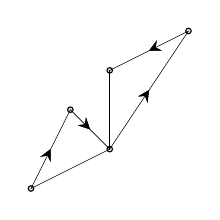
\begin{tikzpicture}[scale=0.5]
    \tkzDefPoint(0,0){v_1}
    \tkzDefPoint(1,2){v_2}
    \tkzDefPoint(2,1){v_3}
    \tkzDefPoint(4,4){v_4}
    \tkzDefPoint(2,3){v_5}
    \tkzDrawPoints(v_1,v_2,v_3,v_4,v_5)
    \tkzDrawSegments[arrowMe=stealth](v_1,v_2 v_2,v_3 v_3,v_4 v_4,v_5)
    \tkzDrawSegments(v_1,v_3 v_3,v_5)
	\end{tikzpicture}\\
	Graf posiada ścieżkę Hamiltona -- zaznaczono ją strzałkami
\end{center}
\end{minipage}
\begin{minipage}{0.5\textwidth}
\begin{center}
	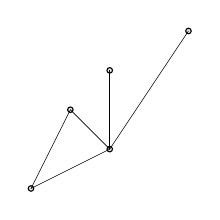
\begin{tikzpicture}[scale=0.5]
    \tkzDefPoint(0,0){v_1}
    \tkzDefPoint(1,2){v_2}
    \tkzDefPoint(2,1){v_3}
    \tkzDefPoint(4,4){v_4}
    \tkzDefPoint(2,3){v_5}
    \tkzDrawPoints(v_1,v_2,v_3,v_4,v_5)
    \tkzDrawSegments(v_1,v_2 v_2,v_3 v_3,v_4)
    \tkzDrawSegments(v_1,v_3 v_3,v_5)
	\end{tikzpicture}\\
	Graf nie posiada ścieżki Hamiltona
\end{center}
\end{minipage}


\vspace{20px}

\heading{Przykład 2}

\noindent
Zdefiniujmy ciąg grafów $(G_n)_{n\geqslant1}$ w następujący sposób.
\begin{itemize}
	\item Graf $G_1$ jest grafem złożonym z dwóch połączonych ze sobą wierzchołków,
	\item Graf $G_{i + 1}$ dla $i \geqslant 2$ otrzymujemy poprzez połączenie dwóch grafów $G_i$, aby każdy wierzchołek z jednego z tych grafów był połączony z dokładnie jednym wierzchołkiem z drugiego z tych grafów.
\end{itemize}

\noindent
Wykazać, że graf $G_{2020}$ ma ścieżkę Hamiltona.

\vspace{5px}

\begin{remark}
Można zauważyć, że $G_n$ to w istocie $n$-wymiarowy hipersześcian.
\end{remark}


\vspace{20px}

\begin{minipage}{0.33\textwidth}
\begin{center}
	\begin{tikzpicture}
    \tkzDefPoint(0,0){v_1}
    \tkzDefPoint(2,0){v_2}
    \tkzDrawPoints(v_1,v_2)
    \tkzDrawSegments(v_1,v_2)
	\end{tikzpicture}\\
	$G_1$
\end{center}
\end{minipage}
\begin{minipage}{0.33\textwidth}
\begin{center}
	\begin{tikzpicture}
    \tkzDefPoint(0,0){v_1}
    \tkzDefPoint(2,0){v_2}
    \tkzDefPoint(2,2){v_3}
    \tkzDefPoint(0,2){v_4}
    \tkzDrawPoints(v_1,v_2, v_3, v_4)
    \tkzDrawSegments(v_1,v_2 v_2,v_3 v_3,v_4 v_1,v_4)
	\end{tikzpicture}\\
	$G_2$
\end{center}
\end{minipage}
\begin{minipage}{0.33\textwidth}
\begin{center}
	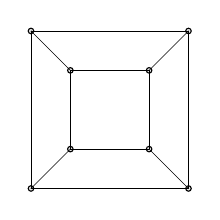
\begin{tikzpicture}
    \tkzDefPoint(0,0){v_1}
    \tkzDefPoint(2,0){v_2}
    \tkzDefPoint(2,2){v_3}
    \tkzDefPoint(0,2){v_4}
    \tkzDefPoint(0.5,0.5){v_5}
    \tkzDefPoint(1.5,0.5){v_6}
    \tkzDefPoint(1.5,1.5){v_7}
    \tkzDefPoint(0.5,1.5){v_8}
    \tkzDrawPoints(v_1,v_2, v_3, v_4)
    \tkzDrawSegments(v_1,v_2 v_2,v_3 v_3,v_4 v_1,v_4)
    \tkzDrawPoints(v_5,v_6, v_7, v_8)
    \tkzDrawSegments(v_5,v_6 v_6,v_7 v_7,v_8 v_5,v_8)
    \tkzDrawSegments(v_5,v_1 v_6,v_2 v_7,v_3 v_8,v_4)
	\end{tikzpicture}\\
	$G_3$
\end{center}
\end{minipage}

\heading{Rozwiązanie}

\noindent
Wykażemy, że teza jest prawdziwa dla każdego $n \geqslant 1$. Co więcej wykażemy, że ścieżka Hamiltona może zaczynać się w każdym z wierzchołków $G_n$.
Zauważmy, że dla $n = 1$ teza jest oczywista -- ścieżka złożona z jednej krawędzi spełnia warunki zadania.

\vspace{10px}

\noindent
Załóżmy, że dla $G_n$ istnieje ścieżka Hamiltona. Wykażemy, że istnieje ona dla $G_{n + 1}$. Graf $G_{n+1}$ składa się z dwóch połączonych ze sobą części izomorficznych z grafem $G_n$ -- nazwijmy je $A$ oraz $B$. Oznaczmy wierzchołki $G_{n + 1}$ kolejno jako
$a_1, a_2, ..., a_{2^n}$ -- cześć $A$ oraz $b_1, b_2, ..., b_{2^n}$ -- część $B$, przy czym $a_i$ jest połączone właśnie z $b_i$. 

\vspace{10px}

\noindent
Ścieżka Hamiltonowska w grafie $G_{n + 1}$ będzie się składać z 3 części:
\begin{itemize}
	\item Na mocy założenia istnieje ścieżka zaczynająca się w $a_1$ przechodząca przez wszystkie wierzchołki $A$. Możemy ją przejść od tyłu. Wówczas przejdziemy wszystkie wierzchołki części $A$ kończąc w $a_1$.
	\item Następnie przejdziemy krawędzią między $a_1$ i $b_1$ do części $B$.
	\item Na mocy założenia z punktu $b_1$ da się poprowadzić ścieżkę, która przejdzie przez każdy z wierzchołków części $B$ dokładnie raz.
\end{itemize}

\noindent
Łatwo zauważyć, że podany sposób przejścia grafu $G_{n + 1}$ tworzy ścieżkę Hamiltonowską.

\qed

\newpage

\begin{problem}{1} 
	Wykazać, że suma miar kątów w $n$-kącie wypukłym wynosi ${(n - 2) \cdot 180\degree}$.
\end{problem}

\begin{problem}{2} 
 Wykazać, że dla każdej dodatniej liczby całkowitej $n$ zachodzi tożsamość
\[
	1^2 + 2^2 + 3^2 + ... + n^2 = \frac{n(n + 1)(2n + 1)}{6}.
\]
\end{problem}

\begin{problem}{3} 
Dana jest następująca gra, zwana \textit{wieżami Hanoi}. Na początku ułożono $n$ dysków na jednej igle tak jak na rysunku. W każdym ruchu gracz może przemieścić dysk na inną igłę, przy czym dysk ten nie może zostać położony na dysk o mniejszej średnicy. Wykazać, że gracz jest w stanie przenieść wszystkie dyski na trzecią igłę.

\begin{center}
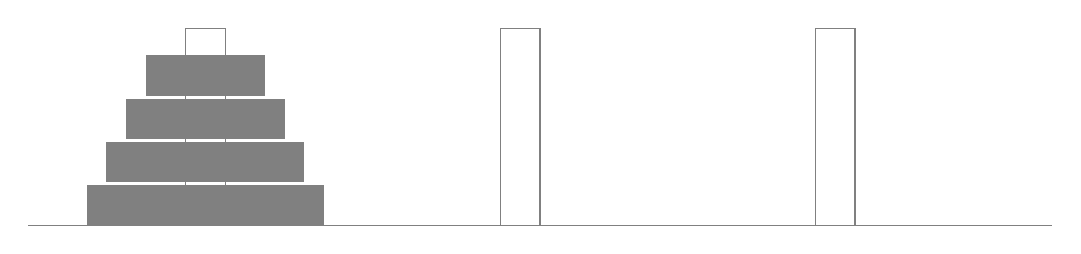
\begin{tikzpicture}[scale=0.5]
	\draw[gray, thin] (0,0) -- (26,0);
	\draw[gray, thin] (4,0) -- (4,5) -- (5,5) -- (5,0);
	\draw[gray, thin] (12,0) -- (12,5) -- (13,5) -- (13,0);
	\draw[gray, thin] (20,0) -- (20,5) -- (21,5) -- (21,0);

	\draw[gray, thin, fill=black!50] (1.5,0) -- (7.5,0) -- (7.5,1) -- (1.5,1) -- cycle;	
	\draw[gray, thin, fill=black!50] (2,1.1) -- (7,1.1) -- (7,2.1) -- (2,2.1) -- cycle;	
	\draw[gray, thin, fill=black!50] (2.5,2.2) -- (6.5,2.2) -- (6.5,3.2) -- (2.5,3.2) -- cycle;	
	\draw[gray, thin, fill=black!50] (3,3.3) -- (6,3.3) -- (6,4.3) -- (3,4.3) -- cycle;
\end{tikzpicture}

\end{center}

\end{problem}

\begin{problem}{4}
	W przestrzeni danych jest $n \geqslant 3$ punktów, że żadne trzy z nich nie leżą na jednej prostej. Każde dwa z tych punktów połączono odcinkiem o kolorze zielonym lub czerwonym. Wykazać, że można wybrać tak jeden z tych kolorów, aby każde dwa z danych punktów były połączone odcinkiem lub łamaną tego koloru.
\end{problem}

\begin{problem}{5} 
Dany jest ciąg liczb rzeczywistych
\[
	a_0 \neq 0, 1,\quad a_1 = 1 - a_0,\quad a_{n + 1} = 1 - a_n(1 - a_n). 
\]
Wykazać, że dla wszystkich $n$ 
\[
	a_0a_1a_2...a_n\left(\frac{1}{a_0} + \frac{1}{a_1} + \frac{1}{a_2} + ... + \frac{1}{a_n}\right) = 1.
\]
\end{problem}

\newpage

\begin{problem}{6} 
	Wykazać, że planszę o wymiarach $2^n \times 2^n$ dla pewnego $n \geqslant 1$ z usuniętym jednym z rogów da się przykryć pewną liczbą L-klocków (takich jak na rysunku). Klocki można obracać.

	\begin{center}
		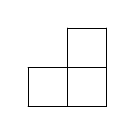
\begin{tikzpicture}[scale=0.5]
	    \tkzDefPoint(0,0){v_1}
	    \tkzDefPoint(2,0){v_2}
	    \tkzDefPoint(2,2){v_3}
	    \tkzDefPoint(1,2){v_4}
	    \tkzDefPoint(1,1){v_5}
	    \tkzDefPoint(0,1){v_6}
	    \tkzDefPoint(1,0){A}
	    \tkzDefPoint(2,1){B}

	    \tkzDrawSegments(v_1,v_2 v_2,v_3 v_3,v_4 v_4,v_5 v_5,v_6  v_6,v_1)
	    \tkzDrawSegments(v_5,A)
	    \tkzDrawSegments(v_5,B)
		\end{tikzpicture}
	\end{center}
\end{problem}

\begin{problem}{7}
Niech $n$ będzie nieparzystą liczbą naturalną, a liczby $x_1,\; x_2,\; ...,\; x_n$ będą parami różne. Dla każdych dwóch liczb $x_i$ oraz $x_j$, gdzie $i > j$, zapisano na tablicy wartość bezwzględną ich różnicy. Wykazać, że można podzielić zapisane liczby na dwa zbiory o równej sumie.
\end{problem}



\newpage
% Rozdział 2 – równania funkcyjne

\theory{Równania funkcyjne}

\heading{Przykład 1}

\noindent
Znajdź wszystkie funkcje $f:\mathbb{R}\rightarrow\mathbb{R}$ spełniające dla wszystkich $x, y \in \mathbb{R}$, równanie 
\[
    f(x + y) = f(x) − f(y).
\]

\heading{Rozwiązanie}

\noindent
Zauważmy, że skoro dane równanie jest spełnione dla wszystkich liczb rzeczywistych $x$~i~$y$ to jest spełnione w szczególności dla $x = y = 0$. Wówczas
\begin{gather*}
    f(0) = f(0) - f(0) = 0.
\end{gather*}

\noindent
Podstawiając do wyjściowej równości $x = 0$ otrzymujemy
\[
    f(y) = f(0) - f(y).
\]
Na mocy wyżej wykazanej zależności $f(y) = 0$ mamy
\begin{gather*}
    f(y) = - f(y) \\
    f(y) = 0.
\end{gather*}
Wykazaliśmy, że $f(x) = 0$ dla wszystkich liczb rzeczywistych $x$. Pozostaje sprawdzić, że istotnie taka funkcja spełnia warunki zadania. Zauważmy, że wówczas
\[
    f(x + y) = 0 = f(x) - f(y).
\]

\qed

\vspace{10px}

\noindent
Metoda polegająca na podstawianiu szczególnych wartości do danego równania jest najważniejszym narzędziem w walce z równaniami funkcyjnymi. Często, aby zadania rozwiązać, należy użyć jej kilka lub nawet kilkanaście razy.

\vspace{10px}

\noindent
Należy zaznaczyć, że bardzo często rozwiązując równanie funkcyjne, wyznacza się zbiór funkcji, które mogą spełniać dane równanie. Jednak często nie oznacza to, że muszą one go spełniać, gdyż podstawianie zazwyczaj nie jest przejściem równoważnym. Dlatego należy zawsze w swoim rozwiązaniu zawrzeć sprawdzenie tego, czy otrzymane funkcje istotnie działają. Brak takiego sprawdzenie w większości przypadków skutkuje obniżeniem oceny za dane zadanie.

\vspace{20px}

\heading{Przykład 2}

\noindent
Znajdź wszystkie funkcje $f:\mathbb{R}\rightarrow\mathbb{R}$ spełniające dla wszystkich $x, y \in \mathbb{R}$ równanie 
\[
    f(2f(x) + f(y)) = 2x + f(y).
\]

\newpage

\heading{Rozwiązanie}

\noindent
Rozwiązanie rozpoczniemy od wykazania następującego lematu.

\vspace{10px}

\noindent
\underline{Lemat 1.} Dla każdego $a \in \mathbb{R}$ istnieje $x \in \mathbb{R}$, że $f(x) = a$.

\vspace{5px}

\noindent
Podstawmy $\dfrac{a - f(y)}{2}$ w miejsce zmiennej $x$
\[
    f\left(f\left(\frac{a - f(y)}{2}\right) + f(y)\right) = 2\left(\frac{a - f(y)}{2}\right) + f(y) = a.
\]

\noindent
Zauważmy, że z otrzymanej równości wynika teza lematu – liczbę $a$ można wybrać dowolnie, zaś po prawej stronie otrzymamy argument, dla którego funkcja przyjmie tę wartość.

\vspace{10px}

\noindent
Korzystając z lematu, podstawmy w miejsce $y$ taką liczbę $a$, aby $f(a) = -2f(x)$. Wówczas
\begin{gather*}
    f(2f(x) + f(a)) = 2x + f(a) \\
     f(0) = 2x - 2f(x) \\
    f(x) = x  + \frac{1}{2}f(0).
\end{gather*}
Podstawiając do powyższej równości $x = 0$ otrzymujemy, że $f(0) = 0$. Stąd
\[
    f(x) = x + \frac{1}{2}f(0) = x.
\]
Sprawdzamy, że funkcja $f(x) = x$ istotnie spełnia warunki zadania.

\qed

\vspace{10px}

\noindent
W powyższym rozumowaniu kluczowe było wykazanie, że dana funkcja przyjmuje wszystkie wartości rzeczywiste -- inaczej mówiąc jest surjekcją. Mogliśmy także wykazać więcej, mianowicie, że dana funkcja jest różnowartościowa. Zakładając, że $f(a) = f(b)$ dla pewnych liczb $a,\;b$ podstawiamy w miejsce $(x, y)$ kolejno $(a, 0)$ i $(b, 0)$ otrzymując
\[
    f(2f(a) + f(y)) = 2a + f(y) \quad \text{oraz} \quad f(2f(b) + f(y)) = 2b + f(y).
\]
Na mocy wyżej założonej równości lewe strony obu zależności są sobie równe. Stąd prawe również, skąd $a = b$. Implikacja $f(a) = f(b) \implies a = b$ jest równoważna temu, że funkcja~$f$ jest różnowartościowa.

\vspace{10px}

\noindent
W większości rozwiązań funkcyjnych konieczne będzie wykonanie wielu ,,sztampowych'' podstawień i spróbować wykazać własności funkcji -- chociażby te wspomniane wyżej. Niekiedy do rozwiązania zadania potrzebny będzie błyskotliwy pomysł czy nietypowe połączenie faktów. W innych zaś przypadkach samo rzetelne i uważne próbowanie znanych trików może okazać się wystarczające. 

\vspace{10px}

\begin{problem}{1} 
	Znajdź wszystkie funkcje $\mathbb{R} \rightarrow \mathbb{R} $ spełniające dla wszystkich $x, y \in \mathbb{R} $ równanie
	\[
		 f(x)+f(y) = f(xy).
	\]
\end{problem}

\begin{problem}{2}
	Znajdź wszystkie funkcje $\mathbb{R} \rightarrow \mathbb{R} $ spełniające dla wszystkich $x, y \in \mathbb{R} $ równanie
	\[
		 f(x-f(y)) = 1 - x - y.
	\]
\end{problem}

\begin{problem}{3}
	Znajdź wszystkie funkcje $\mathbb{R} \rightarrow \mathbb{R} $ spełniające dla wszystkich $x, y \in \mathbb{R} $ równanie 
	\[
		f(x^{2}y) = f(xy) + yf(f(x) + y).
	\]
\end{problem}

\begin{problem}{4}
	Znajdź wszystkie funkcje $\mathbb{R} \rightarrow \mathbb{R} $ spełniające dla wszystkich $x, y \in \mathbb{R} $ równanie 
	\[
		2f(x) + f(1 - x) = x^{2}.
	\] 
\end{problem}

\begin{problem}{5}
	Znajdź wszystkie funkcje $\mathbb{R} \rightarrow \mathbb{R} $ spełniające dla wszystkich $x, y \in \mathbb{R} $ równanie 
	\[
		f(x+y) = f(f(x)) + y + 1.
	\] 
\end{problem}

\begin{problem}{6}
	Znajdź wszystkie funkcje różnowartościowe
	$\mathbb{R} \rightarrow \mathbb{R} $ spełniające dla wszystkich $x, y \in \mathbb{R} $ równość 
	\[
		f(f(x) + y) = f(x+y) + 1.
	\]
\end{problem}

\begin{problem}{7}
	Znajdź wszystkie funkcje 
	$\mathbb{R} \rightarrow \mathbb{R} $ spełniające dla wszystkich $x, y \in \mathbb{R} $ nierówność 
	\[
		f(x^2+y) + f(y) \geqslant f(x^2) + f(x).
	\] 
\end{problem}

\begin{problem}{8}
	Znajdź wszystkie funkcje $\mathbb{Z} \rightarrow \mathbb{Z} $ spełniające dla wszystkich $x \in \mathbb{Z} $ równanie
	\[
		 f(f(x)) =x+1.
	\] 
\end{problem}

\begin{problem}{9}
	Znajdź wszystkie funkcje $\mathbb{R} \rightarrow \mathbb{R} $ spełniające dla wszystkich $x, y \in \mathbb{R} $ równanie 
	\[
		f(x) f(y) = f(x-y).
	\] 
\end{problem}

\begin{problem}{10}
	Udowodnij, że nie istnieje taka funkcja $f:\mathbb{R}\longrightarrow\mathbb{R}$, że dla dowolnych liczb rzeczywistych $x$, $y$ zachodzi równość:
	\[
		f(f(x) + 2f(y)) = x + y.
	\]
\end{problem}



\newpage
% Rozdział 3 – Bijekcje i bajki kombinatoryczne

\theory{Bijekcje i bajki kombinatoryczne}

\noindent
W tym rozdziale będziemy analizować różne zbiory i relacje między nimi. W części zadań trzeba będzie pokazać, że pewne dwa zbiory mają tyle samo elementów. Jedną z metod dowodzenia tego typu stwierdzeń jest połączenie elementów danych zbiorów w pary. Takie przyporządkowanie nazywamy \textit{bijekcją}.

\begin{center}
    \begin{tikzpicture}
        \tkzDefPoint(-1,3){P_0}
        \tkzDefPoint(0,3){P_1}
        \tkzDefPoint(1,3){P_2}
        \tkzDefPoint(2,3){P_3}
        \tkzDefPoint(3,3){P_4}
        \tkzDefPoint(4,3){P_5}
        \tkzDefPoint(5,3){P_6}


        \tkzDefPoint(-1,1){Q_0}
        \tkzDefPoint(0,1){Q_1}
        \tkzDefPoint(1,1){Q_2}
        \tkzDefPoint(2,1){Q_3}
        \tkzDefPoint(3,1){Q_4}
        \tkzDefPoint(4,1){Q_5}
        \tkzDefPoint(5,1){Q_6}

        \tkzDrawSegments[dashed](P_1,Q_1 P_2,Q_2 P_3,Q_3 P_4,Q_4 P_5,Q_5 P_6,Q_6)

        \tkzDrawPoints(P_1, P_2, P_3, P_4, Q_1, Q_2, Q_3, Q_4, P_5, P_6, Q_5, Q_6)

        \tkzLabelPoint[left](P_0){Zbiór $A$}
        \tkzLabelPoint[left](Q_0){Zbiór $B$}
    \end{tikzpicture}
\end{center}

\vspace{10px}

\noindent
Aby stwierdzić czy przyporządkowanie jest bijekcją, wystarczy sprawdzić czy każdy element jednego zbioru jest przyporządkowany do \textit{dokładnie} jednego elementu drugiego zbioru. Poniżej dwa przykłady przyporządkowań, które nie są bijekcjami.

\begin{center}
    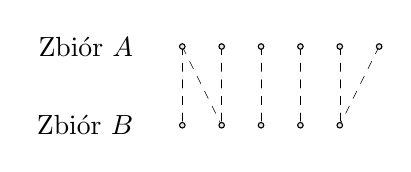
\begin{tikzpicture}[scale=0.5]
        \tkzDefPoint(-1,3){P_0}
        \tkzDefPoint(0,3){P_1}
        \tkzDefPoint(1,3){P_2}
        \tkzDefPoint(2,3){P_3}
        \tkzDefPoint(3,3){P_4}
        \tkzDefPoint(4,3){P_5}
        \tkzDefPoint(5,3){P_6}


        \tkzDefPoint(-1,1){Q_0}
        \tkzDefPoint(0,1){Q_1}
        \tkzDefPoint(1,1){Q_2}
        \tkzDefPoint(2,1){Q_3}
        \tkzDefPoint(3,1){Q_4}
        \tkzDefPoint(4,1){Q_5}
        \tkzDefPoint(5,1){Q_6}

        \tkzDrawSegments[dashed](P_1,Q_1 P_2,Q_2 P_3,Q_3 P_4,Q_4 P_5,Q_5 P_6,Q_5 P_1,Q_2)

        \tkzDrawPoints(P_1, P_2, P_3, P_4, Q_1, Q_2, Q_3, Q_4, P_5, P_6, Q_5)

        \tkzLabelPoint[left](P_0){Zbiór $A$}
        \tkzLabelPoint[left](Q_0){Zbiór $B$}
    \end{tikzpicture}
    \hspace{20px}
    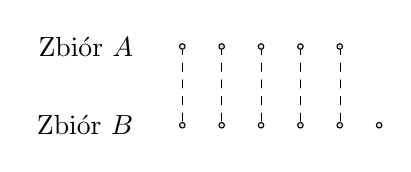
\begin{tikzpicture}[scale=0.5]
        \tkzDefPoint(-1,3){P_0}
        \tkzDefPoint(0,3){P_1}
        \tkzDefPoint(1,3){P_2}
        \tkzDefPoint(2,3){P_3}
        \tkzDefPoint(3,3){P_4}
        \tkzDefPoint(4,3){P_5}
        \tkzDefPoint(5,3){P_6}


        \tkzDefPoint(-1,1){Q_0}
        \tkzDefPoint(0,1){Q_1}
        \tkzDefPoint(1,1){Q_2}
        \tkzDefPoint(2,1){Q_3}
        \tkzDefPoint(3,1){Q_4}
        \tkzDefPoint(4,1){Q_5}
        \tkzDefPoint(5,1){Q_6}

        \tkzDrawSegments[dashed](P_1,Q_1 P_2,Q_2 P_3,Q_3 P_4,Q_4 P_5,Q_5)

        \tkzDrawPoints(P_1, P_2, P_3, P_4, Q_1, Q_2, Q_3, Q_4, P_5, Q_5, Q_6)

        \tkzLabelPoint[left](P_0){Zbiór $A$}
        \tkzLabelPoint[left](Q_0){Zbiór $B$}
    \end{tikzpicture}
\end{center}

\heading{Przykład 1}

\noindent
Dla pewnej liczby całkowitej $n$ jej \textit{podziałem} nazwiemy takie dodatnie liczby całkowite $(a_1, ..., a_t)$, że
\begin{gather*}
    n = a_1 + a_2 + ... + a_t \\
    a_1 \geqslant a_2 \geqslant a_3 \geqslant ... \geqslant a_t \geqslant 0.
\end{gather*}

\noindent
Niech $n$, $k$ będą dodatnimi liczbami całkowitymi. Wykazać, że liczba podziałów $n$, które składają się dokładnie z $k$ liczb jest równa liczbie podziałów $n$, takich, że największy składnik każdego z nich jest równy dokładnie $k$.

\vspace{5px}

\heading{Rozwiązanie}

\vspace{5px}

\noindent
Weźmy dowolny podział liczby $n$. Niech $n = a_1 + a_2 + ... + a_t$. Rozpatrzmy jego reprezentację graficzną zwaną diagramem Ferrera.
Poniżej narysowano diagram Ferrera dla podziału $12 = 4 + 4 + 3 + 1$.
W każdym kolejnym wierszu znajduje się tyle kropek, ile wynosi kolejny składnik z podziału. 

\begin{center}
    \begin{tikzpicture}[scale=0.6]

        \tkzDefPoint(-1,3){A_1}
        \tkzDefPoint(0,3){P_1}
        \tkzDefPoint(1,3){P_2}
        \tkzDefPoint(2,3){P_3}
        \tkzDefPoint(3,3){P_4}


        \tkzDefPoint(-1,2){A_2}
        \tkzDefPoint(0,2){P_5}
        \tkzDefPoint(1,2){P_6}
        \tkzDefPoint(2,2){P_7}
        \tkzDefPoint(3,2){P_8}

        \tkzDefPoint(-1,1){A_3}
        \tkzDefPoint(0,1){P_9}
        \tkzDefPoint(1,1){P_10}
        \tkzDefPoint(2,1){P_11}

        \tkzDefPoint(-1,0){A_4}
        \tkzDefPoint(0,0){P_12}

        \tkzDrawPoints(P_1, P_2, P_3, P_4, P_5, P_6, P_7, P_8, P_9, P_10, P_11, P_12)
        \tkzLabelPoint[left](A_1){4}
        \tkzLabelPoint[left](A_2){4}
        \tkzLabelPoint[left](A_3){3}
        \tkzLabelPoint[left](A_4){1}

        \tkzDefPoint(0,4){B_1}
        \tkzDefPoint(1,4){B_2}
        \tkzDefPoint(2,4){B_3}
        \tkzDefPoint(3,4){B_4}
        \tkzLabelPoint[above](B_1){4}
        \tkzLabelPoint[above](B_2){3}
        \tkzLabelPoint[above](B_3){3}
        \tkzLabelPoint[above](B_4){2}
    \end{tikzpicture}
\end{center}

\noindent
Zastanówmy się, co znaczą założenia zadania w języku rozpatrywanych diagramów.
Jeśli w podziale jest dokładnie $k$ liczb, to diagram Ferrera będzie składał się dokładnie z $k$ wierszy. Jeśli  największy składnik podziału jest równy $k$, to kolumn będzie dokładnie $k$.

\vspace{10px}
\noindent
Zauważmy, że patrząc na dowolny diagram Ferrera ,,od góry'' -- traktujemy kolumny jako wiersze i vice versa -- otrzymamy inny diagram Ferrera. W podanym przykładzie z podziału $12 = 4 + 4 + 3 + 1$ otrzymamy w ten sposób podział $12 = 4 + 3 + 3 + 2$.

\vspace{10px}
\noindent
Jeśli diagram Ferrera przedstawiał podział $n$, który składa się dokładnie z $k$ liczb, to podział otrzymany w powyższy sposób ma największy składnik każdego z nich równy dokładnie $k$. Obie z tych własności są równoważne temu, że diagram na $k$ wierszy.

\vspace{10px}
\noindent
Powyższe przyporządkowanie łączy elementy danych w zadaniu zbiorów w pary -- dokładnie jeden podział pierwszego rodzaju z dokładnie jednym podziałem drugiego rodzaju. Rysując diagram dla pewnego podziału, otrzymamy dokładnie jeden podział z drugiego zbioru, więc to parowanie jest dobre. Stąd wynika, że rozpatrywane zbiory mają tyle samo elementów.

\qed

\vspace{10px}

\noindent
Pokazaliśmy, że pewne dwa zbiory mają tę samą liczbę elementów. Teraz spróbujemy za pomocą kombinatoryki udowodnić równość algebraiczną.

\vspace{5px}


\heading{Przykład 2}

\noindent
Wykazać, że dla wszystkich dodatnich liczb całkowitych $n$, $k$ zachodzi równość
\[
    \sum^{n}_{k=0} {{n}\choose{k}} 2^k = 3^n.
\]

\vspace{5px}

\heading{Rozwiązanie}

\vspace{5px}

\noindent
Na imprezę przyszło $n$ matematyczek. Każda z nich wzięła kapelusz, czapkę lub przyszła bez okrycia głowy. Obliczmy ile różnych wariantów nakryć głowy mogło się zdarzyć na dwa sposoby.
\begin{enumerate}
    \item Każda z dziewczyn mogła wybrać jedną z trzech opcji ubioru, było ich $n$, więc liczba możliwości wynosi $3^n$.
    \item Przyjmijmy, że $n - k$ dziewczyn nie przyniosło żadnego nakrycia głowy. 
    Wówczas możemy wybrać te dziewczyny na ${{n}\choose{n - k}} = {{n}\choose{k}}$ sposobów. 
    Następnie każda z pozostałych $k$ dziewczyn wybrała jedno z dwóch dostępnych nakryć głowy. 
    Więc mogą to zrobić na $2^k$ sposobów. Z reguły mnożenia wynika, że dla ustalonej liczby $k$ jest dokładnie ${{n}\choose{k}} 2^k$ wariantów. Sumując po wszystkich $k$ otrzymujemy $\sum^{n}_{k=0} {{n}\choose{k}} 2^k$.
\end{enumerate}

\noindent
Obliczając jedną rzecz na dwa sposoby otrzymaliśmy liczby, które muszą być równe.

\qed

\vspace{10px}

\noindent
Rozumowania podobne do powyższego nazywane są bajkami kombinatorycznymi.

\vspace{10px}
\begin{problem}{1} 
	Dane są liczby całkowite $n$ i $k$. Wykaż, że
	\[
		\sum^{n}_{k=0} k \cdot {{n}\choose{k}} = n \cdot 2^{n - 1}.
	\]
\end{problem}

\begin{problem}{2}
	Wyznacz liczbę podzbiorów zbioru $\{1, 2, 3, ..., 10\}$, których suma wynosi co najmniej $28$.
\end{problem}

\begin{problem}{3} 
	Udowodnić, że dla wszystkich dodatnich liczb całkowitych $n$ zachodzi równość
	\[
	    \sum^{n}_{k=0} {{n}\choose{k}}^2 = {{2n}\choose{n}}.
	\]
\end{problem}

\begin{problem}{4}
	Dana jest liczba pierwsza $p \geqslant 3$. Niech $A_k$ oznacza zbiór permutacji $(a_1, a_2, ..., a_p)$ zbioru $\{1, 2, 3,..., p\}$, dla których liczba
	\[
		a_1 + 2a_2 + 3a_3 + ... + pa_p - k
	\]
	jest podzielna przez $p$. Wykazać, że zbiory $A_1$ oraz $A_2$ mają tyle samo elementów.
\end{problem}

\begin{problem}{5}
	Wykaż, że dla dowolnych dodatnich liczb całkowitych $n$, $k$ liczba	$(kn)!$
	jest podzielna przez liczbę $(n!)^k \cdot k!$.
\end{problem}


\begin{problem}{6}
	Dana jest liczba całkowita $n$. Niech $T_n$ oznacza liczbę takich podzbiorów zbioru $\{1, 2, 3, ..., n\}$, że ich średnia arytmetyczna jest liczbą całkowitą. Wykazać, że liczba $T_n - n$ jest parzysta.
\end{problem}


\begin{problem}{7}
	Niech $n$, $k$, $r$ będą dodatnimi liczbami całkowitymi. Wykaż, że
	\[
		\sum^{r}_{k=0} {{n + k}\choose{k}} = {{n + r + 1}\choose{r}} .
	\]
\end{problem}



\headingpage{Podpowiedzi 1}
%--------------------------- Hint 1 ---------------------%

\newpage
\hints{Indukcja matematyczna}

\begin{hints_list}
	\item Przeprowadź rozumowanie indukcyjne po liczbie wierzchołków $n$.

	\item Sprawdź, że równość zachodzi dla $n = 1$. Załóż, że równość zachodzi dla $n$ i spróbuj wykazać ją dla $n + 1$.

	\item Przeprowadź indukcję po liczbie $n$. Skorzystaj dla wszystkich początkowych dysków poza najniżej położonym.

	\item Rozpatrz $n + 1$ punktów i zobacz, co się stanie, jeśli usuniemy jeden z nich.

	\item Spróbuj wykazać tezę inducją po $n$. Aby to zrobić, trzeba będzie wykazać indukcyjnie inną równość pomocniczą.

	\item Spróbuj podzielić planszę $2^{n + 1} \cdot 2^{n + 1}$ na kilka części.

	\item Wykaż, że jeśli teza zachodzi dla $n$, to zachodzi również dla $n + 2$.
\end{hints_list}
\hints{Równania funkcyjne}

\begin{hints_list}
	\item Podstaw $y = 0$.
	\item Przyjmij $x = f(y)$.
	\item Wykaż, że $f(0) = 0$.
	\item Podstaw $1 - x$ pod $x$.
	\item Skorzystaj z danego równania dla $x = 0$.
	\item Podstaw $y = -x$.
	\item Przyjmij $x = 0$.
	\item Podstaw $f(x)$ w miejsce $x$.
	\item Podstaw: $x = y = 0$ oraz $x = y$.
	\item Wykaż, że $f$ jest różnowartościowa.
\end{hints_list}
\hints{Bijekcje i bajki kombinatoryczne}

\begin{hints_list}
	\item Na ile sposobów spośród $n$ osób możesz wybrać drużynę i mianować jednego z jej członków kapitanem?
	\item Suma liczb rozpatrywanego zbioru wynosi $55$.
	\item Podzielmy $2n$ osób na dwie grupy po $n$ osób. Załóżmy, że z pierwszej grupy wybieramy $k$ osób. Na ile sposobów możesz to zrobić?
	\item ,,Jeśli pewna permutacja należy do $A_1$, to jeśli pomnożymy wszystkie jej elementy przez $2$, to będzie należała do $A_2$.'' To stwierdzenie nie jest poprawne, ale wyraża pomysł na to zadanie.
	\item Rozpatrz liczbę podziałów $kn$ osób na $k$ grup po $n$ osób. Nie bierz pod uwagę żadnej kolejności grup, ani kolejności osób w grupie. 
	\item Zbiory, których średnia arytmetyczna jest liczbą całkowitą, zawierające więcej niż $1$ element podziel na pary.
	\item Wykaż, że obie strony równości to liczba słów, które składają się z $n + 1$ liter $A$ oraz $r$ liter $B$.
\end{hints_list}

\headingpage{Podpowiedzi 2}
%--------------------------- Hint 2 ---------------------%

\newpage
\hints{Indukcja matematyczna}

\begin{hints_list}

	\item Rozpatrz trójkąt tworzony przez trzy kolejne wierzchołki $n$-kąta.

	\item Odejmij stronami tezę zadania dla $n + 1$ i $n$.

	\item Z założenia indukcyjnego możemy przenieść wszystkie dyski, poza najniżej położonym, na drugą igłę. Należy zauważyć, że dysk, którego nie używamy, nie przeszkodzi w wykonaniu takiego przełożenia.

	\item Co mówi założenie indukcyjne? Rozpatrz przypadek, gdy z usuniętego punktu wychodzą krawędzie różnych kolorów.

	\item Wykaż, że dla każdej liczby $n$ zachodzi równość $a_{n + 1} = 1 - a_0a_1a_2\cdot ... \cdot a_{n}.$.

	\item Podziel planszę na cztery części na pomocą dwóch prostych.

	\item Usuń dwie liczby i skorzystaj z założenia indukcyjnego.
\end{hints_list}
\hints{Równania funkcyjne}

\begin{hints_list}
	\item *
	\item Zauważ, że $f$ jest funkcją liniową.
	\item Podstaw $x = 0$ i $y = - f(0)$.
	\item Otrzymane równanie tworzy z równaniem wyjściowym układ równań.
	\item Wykaż, że $f(x) = x + a$ dla pewnej liczy $a$.
	\item Zauważ, że wartość wyrażania $f(x) - x$ musi być stała. Skorzystaj z różnowartościowości~$f$.
	\item Przyjmij $y = 0$.
	\item Zauważ, że $f(x + 1) = f(f(f(x))) = f(x) + 1$.
	\item Wykonaj podstawienie $x = 0$. Wykaż, że $f(x + y) = f(x - y)$.
	\item Załóż, że $f(a) = f(b)$ i wykaż, że $a = b$.
\end{hints_list}
\hints{Bijekcje i bajki kombinatoryczne}

\begin{hints_list}
	\item Na ile sposobów możesz to zrobić, jeśli założysz, że drużyna składa się z $k$ osób?
	\item Połącz zbiory w pary tak, aby zbiór spełniający warunki zadania był połączony ze zbiorem, który ich nie spełnia.
	\item Zauważ, że ${{n}\choose{k}} = {{n}\choose{n - k}}$.
	\item Znajdź taką funkcję $f$ ze zbioru $\{1, 2, 3,..., p\}$ w zbiór $\{1, 2, 3,..., p\}$, że dla każdego $x$ zachodzi równość $f(x) \equiv 2x \pmod{p}$.
	\item Wykaż, że takich podziałów jest $\dfrac{(kn)!}{(n!)^k \cdot k!}$.
	\item Zauważ, że zbiór może zawierać i nie zawierać swojej średniej arytmetycznej.
	\item Przyjmij, że na miejscu $n + k + 1$ znajduje się ostatnia litera $A$.
\end{hints_list}


\headingpage{Podpowiedzi 3}
%--------------------------- Hint 3 ---------------------%

\newpage
\hints{Indukcja matematyczna}


\begin{hints_list}
	\item Skorzystaj z faktu, że suma kątów w trójkącie wynosi $180\degree$ oraz z założenia indukcyjnego.

	\item *

	\item *

	\item Zauważ, że jeśli z usuniętego punktu wychodzą np. tylko czerwone odcinki, to pomiędzy dowolnymi dwoma punktami da się przejść odcinkami czerwonymi.

	\item Wykaż tezę indukcyjnie za pomocą założenia i udowodnionej równości. Zauważ, że 
	\begin{align*}
		a_0a_1a_2...a_na_{n+1}\left(\frac{1}{a_0} + \frac{1}{a_1} + \frac{1}{a_2} + ... + \frac{1}{a_n} + \frac{1}{a_{n + 1}}\right) = \\ =   a_0a_1a_2...a_na_{n+1}\left(\frac{1}{a_0} + \frac{1}{a_1} + \frac{1}{a_2} + ... + \frac{1}{a_n}\right) + a_0a_1a_2...a_n.
	\end{align*}

	\item Podziel plansze na 1 L-klocek i cztery części, które można pokryć na mocy założenia indukcyjnego.

	\item Zauważ, że suma liczb
	\[
		{x_{2k+3}-x_{2k+1}, \; x_{2k+3}-x_{2k},\; \cdots, \; x_{2k+3}-x_{k+2}} \quad \text{i} \quad {x_{2k+2}-x_{k+1},\; \cdots, \; x_{2k+2}-x_1},
	\]
	jest równa sumie liczb
\begin{gather*}
	x_{2k+3} - x_{2k+2} \quad \text{i} \quad x_{2k+2} - x_{2k+1},\; x_{2k+2} - x_{2k},\; \cdots,\; x_{2k+3} - x_{k+2}  \\ \text{oraz} \quad {x_{2k+3} - x_{k+1},\; \cdots, \; x_{2k+3}-x_1}.
\end{gather*}
\end{hints_list}
\hints{Równania funkcyjne}


\begin{hints_list}
	\item *
	\item Oblicz wartość $f(0)$.
	\item Podstaw $x = 0$.
	\item *
	\item Wstaw $f(x) = x + a$ do wyjściowego równania w celu obliczenia $a$.
	\item Rozumuj podobnie jak w poprzednim zadaniu.
	\item Wywnioskuj z obu nierówności, że $f$ jest funkcją stałą.
	\item Wykaż, że $f(x) = x + f(0)$. W tym celu skorzystaj z całkowitości $x$.
	\item Z tego, że $f(x + y) = f(x - y)$ wywnioskuj, że $f$ jest funkcją stałą.
	\item Zamień $x$ i $y$ miejscami w danym równaniu.
\end{hints_list}
\newpage
\hints{Bijekcje i bajki kombinatoryczne}


\begin{hints_list}
	\item Przesumuj wartość z poprzedniej wskazówki po wszystkich możliwych $k$, aby otrzymać całkowitą liczbę możliwości.
	\item Zauważ, że jeśli zbiór $A$ spełnia warunki zadania, to zbiór $\{1, 2, 3, ..., 10\} - A$ ich nie spełnia.
	\item *
	\item Połącz w pary permutacje $(a_i)$ i $(f(a_i))$. Wykaż, że to parowanie jest poprawne.
	\item Ustaw $kn$ osób w kolejce na $(kn)!$ sposobów, a następnie pierwsze $n$ osób dać do jednej grupy, drugie $n$ osób do drugiej, itd. Z ilu kolejek można uzyskać ten sam podział?
	\item Ile jest rozpatrywanych zbiorów, których nie podzieliliśmy w pary?
	\item *
\end{hints_list}


\headingpage{Rozwiązania}
%--------------------------- Solutions ---------------------%

\newpage
\solutions{Indukcja matematyczna}

\begin{problem}{1} 
	Wykazać, że suma miar kątów w $n$-kącie wypukłym wynosi ${(n - 2) \cdot 180\degree}$.
\end{problem}

\noindent
Zauważmy, że dla $n = 3$ teza jest znanym faktem -- mianowicie suma kątów w trójkącie wynosi $180\degree$.


\begin{center}
	\begin{tikzpicture}[scale=0.6]
		\tkzDefPoint(0,0){A}
		\tkzDefPoint(4,0){B}
		\tkzDefPoint(6,1){C}
		\tkzDefPoint(5,3){D}
		\tkzDefPoint(3,3){E}
		\tkzDefPoint(-1,2){F}
		\tkzDrawSegments(A,B B,C C,D D,E E,F F,A)
		\tkzDrawSegments[dashed](B,D)
		\tkzDrawPoints(A,B,C,D,E,F)
	\end{tikzpicture}
\end{center}

\noindent
Załóżmy, że dla każdego $n$-kąta wypukłego suma jego kątów wynosi ${(n - 2) \cdot 180\degree}$. Rozpatrzmy dowolny $(n+1)$-kąt wypukły. Zauważmy, że ma on więcej niż trzy wierzchołki, więc możemy ,,odciąć'' trójkąt złożony z trzech kolejnych wierzchołków. Podzielimy w ten sposób $(n + 1)$-kąt na $n$-kąt i trójkąt. Korzystając z wypukłości rozpatrywanego wielokąta możemy zauważyć, że suma miar jego kątów wewnętrznych jest sumą miar kątów obu tych wielokątów. Wynosi więc ona
\[
	(n - 2) \cdot 180\degree + 180\degree = (n - 1) \cdot 180\degree,
\]
czego należało dowieść.

\vspace{5px}

\begin{problem}{2}
	 Wykazać, że dla każdej dodatniej liczby całkowitej $n$ zachodzi tożsamość
	\[
		1^2 + 2^2 + 3^2 + ... + n^2 = \frac{n(n + 1)(2n + 1)}{6}.
	\]
\end{problem}

\noindent
Sprawdzamy, że dla $n = 1$ postulowana równość zachodzi.
Załóżmy, że równość
\[
	1^2 + 2^2 + 3^2 + ... + n^2 = \frac{n(n + 1)(2n + 1)}{6}
\]
zachodzi dla pewnej liczby $n$. Chcemy wykazać tezę dla $n + 1$, czyli
\[
	1^2 + 2^2 + 3^2 + ... + n^2 + (n + 1)^2 = \frac{(n + 1)(n + 2)(2n + 3)}{6}.
\]
Zauważmy, że sprowadza się ona do wykazania tożsamości
\[
	\frac{n(n + 1)(2n + 1)}{6} + (n + 1)^2 = \frac{(n + 1)(n + 2)(2n + 3)}{6}.
\]
Przekształcając powyższą równość równoważnie otrzymujemy kolejno
\begin{align*}
	n(n + 1)(2n + 1) + 6(n + 1)^2 &= (n + 1)(n + 2)(2n + 3), \\
	2n^3 + 3n^2 + n + 6(n + 1)^2 &= 2n^3 + 9n^2 + 13n + 6, \\
	6(n + 1)^2 &= 6n^2 + 12n + 6, \\
	(n + 1)^2 &= n^2 + 2n + 1.
\end{align*}

\begin{problem}{3}
Dana jest następująca gra, zwana \textit{wieżami Hanoi}. Na początku ułożono $n$ dysków na jednej igle tak jak na rysunku. W każdym ruchu gracz może przemieścić dysk na inną igłę, przy czym dysk ten nie może zostać położony na dysk o mniejszej średnicy. Wykazać, że gracz jest w stanie przenieść wszystkie dyski na trzecią igłę.

\begin{center}
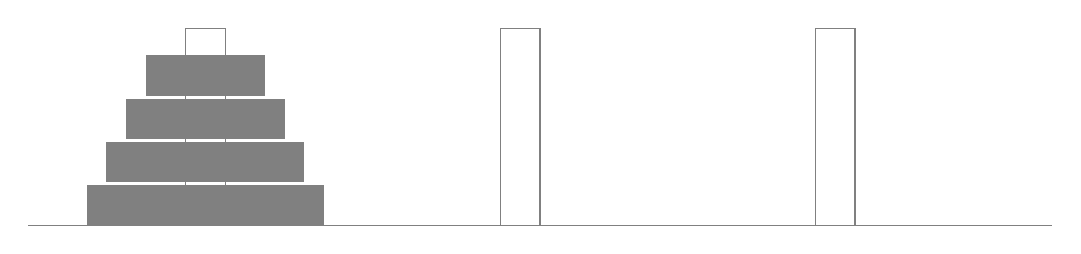
\begin{tikzpicture}[scale=0.5]
	\draw[gray, thin] (0,0) -- (26,0);
	\draw[gray, thin] (4,0) -- (4,5) -- (5,5) -- (5,0);
	\draw[gray, thin] (12,0) -- (12,5) -- (13,5) -- (13,0);
	\draw[gray, thin] (20,0) -- (20,5) -- (21,5) -- (21,0);

	\draw[gray, thin, fill=black!50] (1.5,0) -- (7.5,0) -- (7.5,1) -- (1.5,1) -- cycle;	
	\draw[gray, thin, fill=black!50] (2,1.1) -- (7,1.1) -- (7,2.1) -- (2,2.1) -- cycle;	
	\draw[gray, thin, fill=black!50] (2.5,2.2) -- (6.5,2.2) -- (6.5,3.2) -- (2.5,3.2) -- cycle;	
	\draw[gray, thin, fill=black!50] (3,3.3) -- (6,3.3) -- (6,4.3) -- (3,4.3) -- cycle;
\end{tikzpicture}

\end{center}

\end{problem}

\noindent
Tezę wykażemy indukcją po $n$. Zauważmy, że dla $n = 1$ teza jest oczywista -- wystarczy po prostu przełożyć dysk na trzecią igłę.

\vspace{10px}

\noindent
Załóżmy, że jesteśmy w stanie przełożyć $n - 1$ dysków z pierwszej igły na trzecią. Możemy oczywiście zauważyć, że jest to równoważne chociażby możliwości przełożenia ich z igły pierwszej na drugą.
Przełożenia $n$ dysków dokonujemy w następujący sposób:

\begin{enumerate}
	\item Przekładamy $n - 1$ dysków z góry pierwszej igły na drugą igłę. Zauważmy, że dysk o największym rozmiarze nie przeszkadza nam skorzystać z założenia indukcyjnego, gdyż nie uniemożliwi on wykonania żadnego ruchu.

	\item Dysk pozostawiony na pierwszej igle przekładamy na igłę ostatnią.

	\item Przekładamy $n - 1$ dysków z drugiej igły na trzecią. Analogicznie zauważamy, że obecność jednego dysku na trzeciej igle nie jest problemem.
\end{enumerate}

\begin{problem}{4}
	W przestrzeni danych jest $n \geqslant 3$ punktów, że żadne trzy z nich nie leżą na jednej prostej. Każde dwa z tych punktów połączono odcinkiem o kolorze zielonym lub czerwonym. Wykazać, że można wybrać tak jeden z tych kolorów, aby każde dwa z danych punktów były połączone odcinkiem lub łamaną tego koloru.
\end{problem}

\noindent
Dla $n = 3$ mamy trójkąt. Wybierając kolor, na który pomalowano co najmniej dwa odcinki, postulowana własność będzie spełniona.
\vspace{10px}

\noindent
Załóżmy, że dla teza zachodzi dla $n$ punktów. Rozpatrzmy zbiór $n + 1$ punktów. Wyróżnijmy pewien punkt $P$. Punktów poza $P$ jest dokładnie $n$, więc na mocy założenia istnieje kolor -- bez straty ogólności czerwony -- że pomiędzy każdymi dwoma punktami poza $P$ istnieje łamana tego koloru. 

\begin{minipage}{0.5\textwidth}
\begin{center}
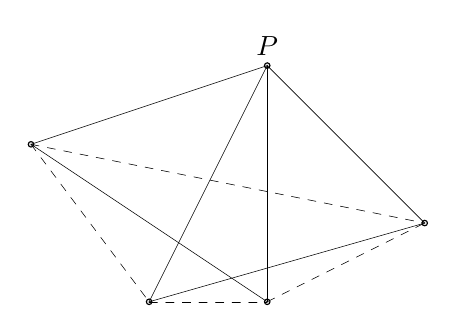
\begin{tikzpicture}
\tkzDefPoint(3,3){P}
\tkzDefPoint(0,2){v_1}
\tkzDefPoint(1.5,0){v_2}
\tkzDefPoint(3,0){v_3}
\tkzDefPoint(5,1){v_4}
\tkzDrawPoints(P, v_1,v_2,v_3,v_4)
\tkzDrawSegments[dashed](v_1,v_2 v_2,v_3 v_3,v_4 v_1,v_4)
\tkzDrawSegments(v_1,v_3 v_2,v_4)
\tkzDrawSegments(P,v_2 P,v_3 P,v_4 v_1,P)
\tkzLabelPoints[above](P)
\end{tikzpicture}\\

\end{center}
\end{minipage}
\begin{minipage}{0.5\textwidth}
\begin{center}
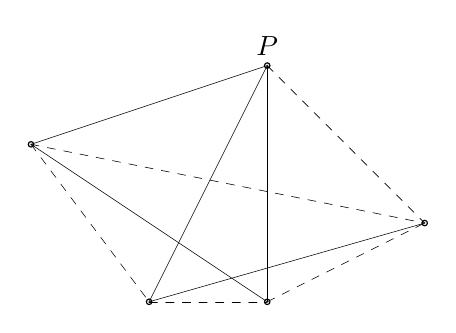
\begin{tikzpicture}
\tkzDefPoint(3,3){P}
\tkzDefPoint(0,2){v_1}
\tkzDefPoint(1.5,0){v_2}
\tkzDefPoint(3,0){v_3}
\tkzDefPoint(5,1){v_4}
\tkzDrawPoints(P, v_1,v_2,v_3,v_4)
\tkzDrawSegments[dashed](v_1,v_2 v_2,v_3 v_3,v_4 v_1,v_4 P,v_4)
\tkzDrawSegments(v_1,v_3 v_2,v_4)
\tkzDrawSegments(P,v_2 P,v_3  v_1,P)
\tkzLabelPoints[above](P)
\end{tikzpicture}\\
\end{center}
\end{minipage}
\begin{center}
Na rysunku zamiast kolorów użyto podziału na linię ciągłą i przerywaną.
\end{center}

Rozpatrzmy dwa przypadki:
\begin{enumerate}
	\item Punkt $P$ jest połączony czerwoną krawędzią z pewnym innym punktem $Q$. Wówczas, wybierając dowolny punkt $X$, na mocy założenia wiemy, że istnieje czerwona ścieżka między $X$ i $Q$. Dokładając do niej odcinek między $P$ i $Q$ otrzymujemy ścieżkę między $P$ oraz $X$.
	Wykazaliśmy, że istnieje ścieżka między punktem $P$ i każdym innym punktem. Łącząc to z faktem, że na mocy założenia indukcyjnego taka ścieżka istnieje między każdą inną parą punktów, otrzymujemy, że dla koloru czerwonego teza jest spełniona.
	\item Punkt $P$ jest połączony z każdym innym punktem niebieskim odcinkiem. Wówczas łatwo zauważyć, że pomiędzy każda parą punktów możemy przejść jednym albo dwoma niebieskimi odcinkami przechodzącymi przez punkt $P$.
\end{enumerate}

\begin{problem}{5}
Dany jest ciąg liczb rzeczywistych
\[
	a_0 \neq 0, 1,\quad a_1 = 1 - a_0,\quad a_{n + 1} = 1 - a_n(1 - a_n). 
\]
Wykazać, że dla wszystkich $n$ 
\[
	a_0a_1a_2...a_n\left(\frac{1}{a_0} + \frac{1}{a_1} + \frac{1}{a_2} + ... + \frac{1}{a_n}\right) = 1.
\]
\end{problem}

\noindent
Na początku wykażemy indukcyjnie, że dla każdego $n$ zachodzi równość
\[
	a_{n + 1} = 1 - a_0a_1a_2\cdot ... \cdot a_{n}.
\]
Równość dla $n = 0$ zachodzi na mocy założeń.
Załóżmy, że
\[
	a_{n} = 1 - a_0a_1a_2\cdot ... \cdot a_{n - 1}.
\]
Skoro $a_{n + 1} = 1 - a_n(1 - a_n)$, to otrzymujemy
\[
	a_{n + 1} = 1 - a_n(1 - a_n) = 1 - a_n \cdot a_0a_1a_2\cdot ... \cdot a_{n - 1} = 1 - a_0a_1a_2\cdot ... \cdot a_{n}.
\]
Więc na mocy zasady indukcji matematycznej postulowana równość zachodzi.
\vspace{10px}

\noindent
Teraz przejdziemy do udowodnienia tezy.
Dla $n = 1$ jest ona oczywista.
Załóżmy, że zachodzi równość
\[
	a_0a_1a_2...a_n\left(\frac{1}{a_0} + \frac{1}{a_1} + \frac{1}{a_2} + ... + \frac{1}{a_n}\right) = 1.
\]
Chcemy wykazać, że
\[
	a_0a_1a_2...a_na_{n+1}\left(\frac{1}{a_0} + \frac{1}{a_1} + \frac{1}{a_2} + ... + \frac{1}{a_n} + \frac{1}{a_{n + 1}}\right) = 1.
\]
Przekształcamy powyższą równość korzystając z założenia
\begin{multline*}
	a_0a_1a_2...a_na_{n+1}\left(\frac{1}{a_0} + \frac{1}{a_1} + \frac{1}{a_2} + \frac{1}{a_3} + ... + \frac{1}{a_n} + \frac{1}{a_{n + 1}}\right) = \\ = a_{n+1} \cdot a_0a_1a_2...a_n\left(\frac{1}{a_0} + \frac{1}{a_1} + \frac{1}{a_2} + ... + \frac{1}{a_n}\right) + a_0a_1a_2...a_n = \\ = a_{n + 1} + a_0a_1a_2...a_n = 1 - a_0a_1a_2...a_n + a_0a_1a_2...a_n = 1.
\end{multline*}

\begin{problem}{6}
	Wykazać, że planszę o wymiarach $2^n \times 2^n$ dla pewnego $n \geqslant 1$ z usuniętym jednym z rogów da się przykryć pewną liczbą $L$ klocków(takich jak na rysunku). Klocki można obracać.

	\begin{center}
		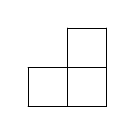
\begin{tikzpicture}[scale=0.5]
	    \tkzDefPoint(0,0){v_1}
	    \tkzDefPoint(2,0){v_2}
	    \tkzDefPoint(2,2){v_3}
	    \tkzDefPoint(1,2){v_4}
	    \tkzDefPoint(1,1){v_5}
	    \tkzDefPoint(0,1){v_6}
	    \tkzDefPoint(1,0){A}
	    \tkzDefPoint(2,1){B}

	    \tkzDrawSegments(v_1,v_2 v_2,v_3 v_3,v_4 v_4,v_5 v_5,v_6  v_6,v_1)
	    \tkzDrawSegments(v_5,A)
	    \tkzDrawSegments(v_5,B)
		\end{tikzpicture}
	\end{center}
\end{problem}

\noindent
Zauważmy, że plansza $2\times2$ z usuniętym rogiem jest w istocie L-klockiem, więc da się ją pokryć.

\begin{center}
	\begin{tikzpicture}[scale=0.3]
    \tkzDefPoint(0,0){A}
    \tkzDefPoint(0,10){B}
    \tkzDefPoint(10,10){C}
    \tkzDefPoint(10,0){D}
    \tkzDefPoint(9,0){P1}
    \tkzDefPoint(9,1){P2}
    \tkzDefPoint(10,1){P3}
    \tkzDrawSegments(A,B B,C C,D D,A)
    \tkzDrawSegments(P2,P1 P3,P2)


    \tkzDefPoint(5,0){G1}
    \tkzDefPoint(5,10){G2}
    \tkzDefPoint(0,5){G3}
    \tkzDefPoint(10,5){G4}
    \tkzDrawSegments(G1,G2 G3,G4)

    \tkzDefPoint(4,4){T1}
    \tkzDefPoint(4,6){T2}
    \tkzDefPoint(6,6){T3}
    \tkzDefPoint(6,5){T4}
    \tkzDefPoint(5,4){T5}
    \tkzDrawSegments(T1,T2 T2,T3 T3,T4 T1,T5) 
	\end{tikzpicture}\\
\end{center}

\noindent
Załóżmy, że dla planszy $2^{n - 1} \times 2^{n - 1}$ istnieje szukane pokrycie. Pokrycie dla planszy $2^{n} \times 2^{n}$ konstruujemy następująco. Dzielimy planszę dwiema prostymi na trzy jednakowe części i czwartą taką samą, tylko bez rogu. Kładziemy jeden klocek na środku, tak jak na rysunku. Wówczas plansza jest podzielona na cztery jednakowe puste części, które na mocy założenia indukcyjnego można pokryć.

\begin{problem}{7}
Niech $n$ będzie nieparzystą liczbą naturalną, a liczby $x_1,\; x_2,\; ...,\; x_n$ będa parami różne. Dla każdych dwóch liczb $x_i$ oraz $x_j$ zapisano na tablicy wartość bezwzględną ich różnicy. Wykazać, że można podzielić zapisane liczby na dwa zbiory o równej sumie.
\end{problem}
\noindent
Przez multizbiór rozumiemy zbiór w którym jeden element może występować kilka razy.
Załóżmy, że $x_1 \geqslant x_2 \geqslant ... \geqslant x_n$. 
\vspace{10px}

\noindent
Wykażemy tezę dla $n = 3$. Podział na zbiory $\{x_1 - x_2, x_2 - x_3\}$ oraz $\{x_1 - x_3\}$ spełnia warunki zadania.
\vspace{10px}

\noindent
Załóżmy, że teza zachodzi dla $2n + 1$, wykażemy ją dla $2n + 3$.
Rozpatrzmy szukany podział multizbioru różnic zbioru $\{x_1, x_2, ..., x_{2n + 1}\}$ na multizbiory $A$ i $B$ o równej sumie elementów.
Dorzucamy do multizbioru $A$ liczby
\[
	{x_{2k+3}-x_{2k+1}, \; x_{2k+3}-x_{2k},\; \cdots, \; x_{2k+3}-x_{k+2}} \quad \text{i} \quad {x_{2k+2}-x_{k+1},\; \cdots, \; x_{2k+2}-x_1},
\]
a do multizbioru $B$ liczby
\begin{gather*}
	x_{2k+3} - x_{2k+2} \quad \text{i} \quad x_{2k+2} - x_{2k+1},\; x_{2k+2} - x_{2k},\; \cdots,\; x_{2k+3} - x_{k+2}  \\ \text{oraz} \quad {x_{2k+3} - x_{k+1},\; \cdots, \; x_{2k+3}-x_1}.
\end{gather*}
Łatwo sprawdzić, że suma dorzuconych elementów jest równa. Stąd wynika, że otrzymane zbiory również mają równą sumę elementów, co jest równoważne tezie.
\newpage
\solutions{Równania funkcyjne}

\begin{problem}{1} 
	Znajdź wszystkie funkcje $\mathbb{R} \rightarrow \mathbb{R} $ spełniające dla wszystkich $x, y \in \mathbb{R} $ równanie
	\[
		 f(x)+f(y) = f(xy).
	\]
\end{problem}

\answer{Jedyną funkcją spełniającą warunki zadania jest $f(x) = 0$.}

\noindent
Podstawmy $y=0$: \[ f(x) + f(0) = f(0), \] czyli $f(x) = 0 $ dla każdego x. Łatwo sprawdzić, że ta funkcja spełnia warunki zadania. 

\vspace{10px}

\begin{problem}{2}
	Znajdź wszystkie funkcje $\mathbb{R} \rightarrow \mathbb{R} $ spełniające dla wszystkich $x, y \in \mathbb{R} $ równanie
	\[
		 f(x-f(y)) = 1 - x - y.
	\]
\end{problem}

\noindent
Podstawmy $x = f(y)$. Otrzymamy 
\begin{gather*}
	f(0) = 1 - f(y) - y, \\
	f(y) = - y + (1 - f(0)).
\end{gather*} 
Podstawmy $y = 0$ do powyższej zależności. Wówczas łatwo obliczyć, że $f(0)=\frac{1}{2}$. Czyli $f(x) = - x + \frac{1}{2} $. Ta funkcja istotnie spełnia warunki zadania, gdyż
\[
	f(x - f(y)) = f(y) - x + \frac{1}{2} = 1 - y - x .
\]

\begin{problem}{3}
	Znajdź wszystkie funkcje $\mathbb{R} \rightarrow \mathbb{R} $ spełniające dla wszystkich $x, y \in \mathbb{R} $ równanie 
	\[
		f(x^{2}y) = f(xy) + yf(f(x) + y).
	\]
\end{problem}

\answer{Funkcja $f(x) = 0$ jest jedynym rozwiązaniem.}

\noindent
Podstawmy $x = 0$ i $y = -f(0)$. Otrzymamy $f(0)^{2}=0$, czyli $f(0)=0$. Podstawmy $x=0$: 
\[ 
	0 = yf(f(0) + y) = yf(y)
\] 
Dla niezerowego $y$ mamy $f(y) = 0$.
Sprawdzamy, że funkcja $f(x) = 0$ spełnia warunki zadania. Łącząc powyższe wnioski otrzymujemy, że jedynie funkcja $f(x)=0$ spełnia warunki zadania. 

\newpage

\begin{problem}{4}
	Znajdź wszystkie funkcje $\mathbb{R} \rightarrow \mathbb{R} $ spełniające dla wszystkich $x, y \in \mathbb{R} $ równanie 
	\[
		2f(x) + f(1 - x) = x^{2}.
	\] 
\end{problem}

\answer{Jedyną funkcją spełniającą warunki zadania jest $f(x) = \frac{2x^2 - (1-x)^2}{3}$.}

\noindent
Podstawmy $1-x$ za x. Otrzymamy 
\[ 
	2f(1 - x) + f(x) = 2(1 - x)^{2}.
\] 
Z równaniem z zadania tworzy to układ równań ze zmiennymi $f(x)$ i $f(1 - x)$. Wyliczamy $f(x) = \frac{2x^{2}-(1-x)^{2}} {3} $. Wystarczy teraz tylko sprawdzić, że ta funkcja spełnia warunki zadania. 

\vspace{5px}

\begin{problem}{5}
	Znajdź wszystkie funkcje $\mathbb{R} \rightarrow \mathbb{R} $ spełniające dla wszystkich $x, y \in \mathbb{R} $ równanie 
	\[
		f(x+y) = f(f(x)) + y + 1.
	\] 
\end{problem}

\answer{$f(x) = x - 1$ jest jedynym rozwiązaniem danego równania.}

\noindent
Podstawmy $x = 0$: 
\[
 f(y) = f(f(0)) + 1 + y, 
\] 
czyli $f(x) = x + a$ dla pewnego stałego $a$. Podstawmy tę funkcję do wyjściowego równania
\[
	x+y+a=x+2a+y+1.
\] 
Mamy $a = -1$. Łatwo sprawdzić, że funkcja $f(x) = x - 1$ spełnia warunki zadania. 

\vspace{5px}

\begin{problem}{6}
	Znajdź wszystkie funkcje różnowartościowe
	$\mathbb{R} \rightarrow \mathbb{R} $ spełniające dla wszystkich $x, y \in \mathbb{R} $ równość 
	\[
		f(f(x) + y) = f(x+y) + 1.
	\]
\end{problem}

\answer{Jedyną funkcją spełniającą warunki zadania jest $f(x) = x + 1$.}

\noindent
Podstawmy $y = -x$. Otrzymamy 
\[ 
	f(f(x) - x) = f(0) + 1.
\] 
Zauważmy, że prawa strona równości jest stała. Z różnowartościowości f wynika, że wartość $f(x) - x$ jest stała. Czyli $f(x) - x = a$ dla pewnego $a$. Wstawiamy $f(x) = x + a$ do wyjściowego równania 
\[
	x + y + 2a = x + y + a + 1,
\]
więc $a = 1$. Skąd $f(x) = x + 1 $ -- możemy sprawdzić, że ta funkcja spełnia warunki zadania.

\newpage

\begin{problem}{7}
	Znajdź wszystkie funkcje 
	$\mathbb{R} \rightarrow \mathbb{R} $ spełniające dla wszystkich $x, y \in \mathbb{R} $ nierówność 
	\[
		f(x^2+y) + f(y) \geqslant f(x^2) + f(x).
	\] 
\end{problem}

\noindent
Podstawmy $x = 0$
\[ 
	f(y) \geqslant f(0). 
\] 
Podstawmy $y = 0$ 
\[ 
	f(x^2) + f(0) \geqslant f(x^2) + f(x), 
\] 
czyli $f(0) \geqslant f(x) $. 
Łącząc oba wnioski otrzymujemy
\[ 
	f(0) \geqslant f(x) \geqslant f(0), 
\] 
czyli $f(x) = f(0)$. Innymi słowy $f$ jest funkcją stałą. Łatwo zauważyć, że taka funkcja spełnia warunki zadania. 

\vspace{5px}

\begin{problem}{8}
	Znajdź wszystkie funkcje $\mathbb{Z} \rightarrow \mathbb{Z} $ spełniające dla wszystkich $x \in \mathbb{Z} $ równanie
	\[
		 f(f(x)) =x+1.
	\] 
\end{problem}

\answer{Szukane funkcje nie istnieją.}

\noindent
Zauważmy, że zachodzą równości 
\begin{gather*} 
f(f(f(x))) = f(x + 1) \\
f(f(f(x))) = f(x) +1 
\end{gather*} 
Z tego otrzymujemy równość: 
\[
	f(x) =f(x-1)+1 
\] 
Skoro działamy w liczbach całkowitych to możemy wywnioskować, że
\[
	f(x) = f(x - 1) + 1 = f(x - 2) +  2 =  ... = x + f(0).
\] 
Podstawmy równość $f(x) = x + f(0)$ do 
$f(f(x)) = x + 1$:
\[
	x + 1 = f(f(x))= x + 2f(0), 
\]
czyli $f(0) = \frac{1}{2}$. Sprzeczność. Takie funkcje nie istnieją.

\vspace{5px} 

\begin{problem}{9}
	Znajdź wszystkie funkcje $\mathbb{R} \rightarrow \mathbb{R} $ spełniające dla wszystkich $x, y \in \mathbb{R} $ równanie 
	\[
		f(x) f(y) = f(x-y).
	\] 
\end{problem}

\answer{Daną zależność spełniają funkcje $f(x) = 1$ i $f(x) = 0$.}

\noindent
Podstawmy $x = y = 0$. Wtedy otrzymujemy 
\[
	f(0)^{2} = f(0) \implies f(0) \in \{0, 1\}.
\]
Podstawmy $x = y$
\[
	f(x)^{2} = f(0).
\] 
Jeśli $f(0)=0$, to $f(x) =0$. Łatwo sprawdzić, że funkcja zerowa spełnia warunki zadania.
Zobaczmy, co jeśli $x = y$ oraz $f(0) = 1$:
\[
	f(x)^{2} = f(0) = 1 
\] 
Czyli $f(x)$ jest równe $-1$ lub 1 dla każdego $x$.
Podstawmy $x=0$
\[
	f(y) =f(-y).
\] 
Zauważmy, że 
\[
	f(x - y) = f(x)f(y) = f(x)f(-y) = f(x+y). 
\] 
Weźmy 2 dowolne liczby a i b. Biorąc $x=\frac{a+b}{2}$ oraz 
$y=\frac{a-b}{2}$ otrzymamy
\[
	f(x+y) = f(x-y) \implies f(a) = f(b).
\] 
Skoro $a$ i $b$ były dowolne to $f$ jest funkcją stałą, czyli $f(x) = 1$. Łatwo sprawdzić, że ta funkcja również spełnia warunki zadania. Czyli tę zależność spełniają funkcje $f(x) = 1 $ i $f(x) = 0$. Sprawdzamy, że istotnie one działają.

\vspace{5px}

\begin{problem}{10}
	Udowodnij, że nie istnieje taka funkcja $f:\mathbb{R}\longrightarrow\mathbb{R}$, że dla dowolnych liczb rzeczywistych $x$, $y$ zachodzi równość:
	\[
		f(f(x) + 2f(y)) = x + y.
	\]
\end{problem}

\noindent
\underline{Lemat 1} Funkcja $f$ jest różnowartościowa

\vspace{10px}
\noindent
Załóżmy, że $f(a) = f(b)$. Podstawmy, $x=a$ oraz $x = b$
\[
	f(f(a) + 2f(y)) = a + y \quad \text{oraz} \quad f(f(b) + 2f(y)) = b + y.
\] 
Skoro $f(a)=f(b)$, to 
\[
	f(f(a) + 2f(y)) = f(f(b) + 2f(y)),
\] 
a więc $a + y = b + y$, czyli $a = b$. A więc $f$ istotnie jest różnowartościowa.
\vspace{10px}

\noindent
Zauważamy, że zachodzą równości
\[
	f(f(x) + 2f(y)) = x + y \quad \text{oraz} \quad f(f(y)+2f(x))=x+y.
\]
Czyli 
\[
	f(f(x) + 2f(y)) = f(f(y) + 2f(x)).
\] 
Skoro $f$ jest różnowartościowa, to 
\[
	f(x)+2f(y)=f(y)+2f(x),
\]
więc $f(x)=f(y)$ dla wszystkich liczb $x$, $y$. Czyli $f$ musiałaby być funkcją stałą, a to jest oczywista sprzeczność z danym równaniem.

\newpage
\solutions{Bijekcje i bajki kombinatoryczne}


\begin{problem}{1} 
	Dane są liczby całkowite $n$ i $k$. Wykaż, że
	\[
		\sum^{n}_{k=0} k \cdot {{n}\choose{k}} = n \cdot 2^{n - 1}.
	\]
\end{problem}

\vspace{5px}

\noindent
Spośród $n$ osób będziemy chcieli wybrać drużynę i mianować jednego jej członka kapitanem. Wykażemy, że wyrażenia po obu stronach równości są liczbą możliwości takiego wyboru.

\vspace{10px}
\noindent
Wybierając najpierw kapitana -- możemy go wybrać na $n$ sposobów -- a następnie dobierając mu zawodników -- których można wybrać na $2^{n - 1}$ sposobów, gdyż wybieramy dowolny podzbiór $n - 1$ osób -- otrzymamy $n \cdot 2^{n - 1}$ osób.

\vspace{10px}
\noindent
Przyjmijmy, że w drużynie wraz z kapitanem jest $k$ osób. Możliwości wyboru $k$ osób spośród $n$ jest ${n}\choose{k}$, a opcji wyboru kapitana spośród tych $k$ osób jest dokładnie $k$. Stąd też dla dowolnego $k$ liczba wariantów wynosi $k \cdot {{n}\choose{k}} $. Sumując po wszystkich możliwych $k$ otrzymujemy, że łączna liczba możliwości wynosi $\sum^{n}_{k=0} k \cdot {{n}\choose{k}}$.

\vspace{5px}

\begin{problem}{2}
	Wyznacz liczbę podzbiorów zbioru $\{1, 2, 3, ..., 10\}$, których suma wynosi co najmniej $28$.
\end{problem}

\vspace{5px}

\answer{Szukana liczba podzbiorów wynosi $2^9 = 512$.}

\noindent
Zauważmy, że suma wszystkich elementów tego zbioru wynosi $55$. Dla każdego podzbioru $A$ zdefiniujmy jego dopełnienie jako podzbiór $\{1, 2, 3, ..., 10\} - A$. Składa się on z wszystkich elementów nie występujących w $A$. Dla przykładu dopełnieniem zbioru $\{1, 2, 4, 7, 8, 9\}$ będzie zbiór $\{3, 5, 6, 10\}$.
\vspace{10px}

\noindent
Zauważmy, że suma elementów dowolnego podzbioru i jego dopełnienia wynosi $55$. Więc dokładnie jeden z tych zbiorów ma sumę elementów większą lub równą $28$. Podzielmy wszystkie rozpatrywane podzbiory na pary zawierające dwa zbiory będące swoim dopełnieniem. Z powyższej obserwacji wynika, że dokładnie połowa podzbiorów -- po jednym z każdej pary -- będzie spełniać warunki zadania. Jest więc ich $\frac{1}{2} \cdot 2^{10} = 2^9 = 512$.


\newpage

\begin{problem}{3} 
	Udowodnić, że dla wszystkich dodatnich liczb całkowitych $n$ zachodzi równość
	\[
	    \sum^{n}_{k=0} {{n}\choose{k}}^2 = {{2n}\choose{n}}.
	\]
\end{problem}

\vspace{5px}

\noindent
Prawa strona równości jest równa liczbie sposobów wyboru $n$ spośród $2n$ osób.
\vspace{10px}

\noindent
Podzielmy te $2n$ osób na dwie grupy po $n$ osób. Załóżmy, że z pierwszej grupy wybieramy $k$ osób. Możemy tego dokonać na ${n}\choose{k}$ sposobów. Z drugiej grupy wybieramy $n - k$ osób -- mamy ${{n}\choose{n - k}} = {{n}\choose{k}}$ możliwości. Dla ustalonego $k$ możemy dokonać wyboru na ${{n}\choose{k}}^2$ sposobów. Sumując po wszystkich $k$ otrzymujemy lewą stronę równości.

\begin{problem}{4}
	Dana jest liczba pierwsza $p \geqslant 3$. Niech $A_k$ oznacza zbiór permutacji $(a_1, a_2, ..., a_p)$ zbioru $\{1, 2, 3,..., p\}$, dla których liczba
	\[
		a_1 + 2a_2 + 3a_3 + ... + pa_p - k
	\]
	jest podzielna przez $p$. Wykazać, że zbiory $A_1$ oraz $A_2$ mają tyle samo elementów.
\end{problem}

\vspace{5px}

\noindent
Ideą poniższego rozwiązania jest fakt, że jak mamy pewną permutację z $A_1$, pomnożymy każdy jej z elementów przez 2, to otrzymamy permutację z $A_2$. Jako, że mnożąc liczbę większą od $\frac{1}{2}p$ przez $2$ wylecimy ze zbioru $\{1, 2, 3,..., p\}$ to zamiast mnożenia przez $2$ użyjemy funkcji danej wzorem
\[
	f(x) = 
	\begin{cases}
	2x \;\;\; \quad\quad\text{dla} \;\; x < \frac{1}{2}p\\
	2x - p \quad \text{dla} \;\; x > \frac{1}{2}p.
	\end{cases}
\]
Zauważmy, że $f(x) \equiv 2x \pmod{p}$.
\vspace{10px}

\noindent
W ten sposób przyporządkujemy każdemu elementowi ze zbioru $A_1$ dokładnie 1 element ze zbioru $A_2$. Czy może się jednak tak zdarzyć, że pewien element z $A_2$ zostanie w ten sposób przyporządkowany nie do jednego, a do innej liczby elementów z $A_1$? Wykażemy, że nie.
\vspace{10px}

\noindent
Mianowicie pokażemy, że z dowolnego elementu $A_2$ możemy odzyskać dokładnie jedną przyporządkowaną mu permutację z $A_1$. Zdefiniujmy ,,dzielenie przez $2$ modulo $p$'' wzorem
\[
	g(x) = 
	\begin{cases}
	\frac{1}{2}x \;\; \quad\quad\quad\text{dla x parzystych}\\
	\frac{1}{2}(x - p) \quad \text{dla x nieparzystych}.
	\end{cases}
\]
Mamy $2g(x) \equiv x \pmod{p}$.
Zauważmy, że jest to funkcja odwrotna do $f$ -- tj. $f(g(x)) = x$.
\vspace{10px}

\noindent
Zauważmy, że
\[
	(a_1, a_2, ..., a_p) \in A_2 \iff (g(a_1), g(a_2), ..., g(a_p)) \in A_1.
\] 
Pozostaje zauważyć, że to permutacja $(a_i)$ była przyporządkowana do permutacji~$(g(a_i))$. Jest tak, bo $f(g(a_i)) = a_i$. Stąd podane parowanie było poprawne, czyli istotnie zbiory $A_1$ i $A_2$ są równoliczne.
\vspace{10px}

\remark{Kluczowym faktem w powyższym rozumowaniu było istnienie funkcji odwrotnej do funkcji $f$ zdefiniowanej dla każdego elementu zbioru $\{1, 2, ..., p\}$.} 

\vspace{5px}

\begin{problem}{5}
	Wykaż, że dla dowolnych dodatnich liczb całkowitych $n$, $k$ liczba	(kn)!
	jest podzielna przez liczbę $(n!)^k \cdot k!$.
\end{problem}

\vspace{5px}

\noindent
Rozpatrzmy liczbę podziałów $kn$ osób na $k$ grup po $n$ osób. Nie bierzemy pod uwagę żadnej kolejności grup, ani kolejności osób w grupie. 

\vspace{10px}
\noindent
Możemy ustawić $kn$ osób w kolejce na $(kn)!$ sposobów, a następnie pierwsze $n$ osób dać do jednej grupy, drugie $n$ osób do drugiej, itd. 

\vspace{10px}
\noindent
Każdą z $k$ grup możemy ustawić w kolejności na $n!$ sposobów. Te grupy możemy ustawić w kolejności na $k!$ sposobów. W ten sposób z jednego podziału na grupy możemy uzyskać dokładnie $(n!)^k \cdot k!$ kolejek. 

\vspace{10px}
\noindent
Więc liczba podziałów na grupy wynosi $\frac{(kn)!}{(n!)^k \cdot k!}$. Skoro jest ona całkowita, to musi zachodzić rozpatrywana podzielność.

\vspace{5px}



\begin{problem}{6}
	Dana jest liczba całkowita $n$. Niech $T_n$ oznacza liczbę takich podzbiorów zbioru $\{1, 2, 3, ..., n\}$, że ich średnia arytmetyczna jest liczbą całkowitą. Wykazać, że liczba $T_n - n$ jest parzysta.
\end{problem}

\vspace{5px}

\noindent
Zauważmy, że zbiory, których średnia arytmetyczna jest liczbą całkowitą, zawierające więcej niż $1$ element da się podzielić na pary. Mianowicie zbiory $S$ i $S'$ o średniej arytmetycznej elementów równej $a$ będą w jednej parze jeśli jeden z tych zbiorów zawiera $a$, drugi nie zawiera, a poza tym mają te same elementy.

$T_n$ będzie takiej parzystości jak liczba niesparowanych zbiorów. Są to wszystkie zbiory jednoelementowe -- jest ich $n$.  Stąd $T_n - n$ jest liczba parzystą.

\vspace{5px}

\begin{problem}{7}
	Niech $n$, $k$, $r$ będą dodatnimi liczbami całkowitymi. Wykaż, że
	\[
		\sum^{r}_{k=0} {{n + k}\choose{k}} = {{n + r + 1}\choose{r}} .
	\]
\end{problem}

\vspace{5px}

\noindent
Wykażemy, że obie strony równości to liczba słów, które składają się z $n + 1$ liter $A$ oraz $r$ liter $B$. Z jednej strony możemy wybrać na $r$ sposobów pozycje liter $B$, a na pozostałych miejscach ustawić litery $A$. Stąd tych słów jest ${{n + r + 1}\choose{r}}$.

Przyjmijmy, że na miejscu $n + k + 1$ znajduje się ostatnia litera $A$. Na $n + k$ poprzednich miejsc znajdzie się $n$ liter $A$ i $k$ liter $B$. Możemy je więc ustawić na ${{n + k}\choose{k}}$ sposobów. Po ostatniej literze $A$ będą same litery $B$, więc nie mamy wyboru. Stąd dla ustalonego $k$ jest ${{n + k}\choose{k}}$ sposobów. Sumując po wszystkich możliwych $k$ otrzymujemy lewą stronę równości.



\end{document}